\documentclass[../main_proj5.tex]{subfiles}

\graphicspath{{\subfix{Figures/}}}

\begin{document}

\begin{figure*}[ht!]
    \centering
    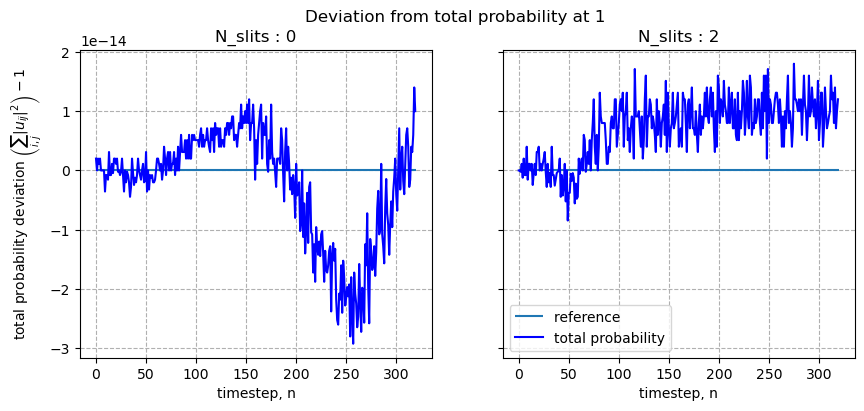
\includegraphics[width=0.8\linewidth]{Project 5/figures/problem7_M201_Nslits0_N_slits2_tot_prob.png}
    \caption{The deviation from a total probability of 1.0 as a function of the time step. The left panel show the stability with no middle wall while the right hand panel use a double slit.}
    \label{fig:p5_computational_stability}
\end{figure*}

\section{Results and discussion}\label{sec:p5_results_and_discussion}

\subsection{Numerical stability}

To investigate the numerical stability of our implementation we simulated with no middle wall and 2 slit wall for $T=0.008$ which implies $N_t = 320$ time steps, that is we conduct the numerical stability experiment. Figure \ref{fig:p5_computational_stability} show the deviation from a total probability of 1.0 as a function of the time step. To complement the Figure the simulation animation is found in the project git directory: \href{https://github.uio.no/johannlf/FYS3150/tree/main/Project5/Results/Problem%207/gifs}{/Project5/Results/Problem7/gifs}. 



Figure \ref{fig:p5_computational_stability} show only small deviations over the 320 time steps with a maximum deviation on the order of $10^{-14}$. Given the maximum precision for double in c++ on the order of $10^{-15}$ (found by running \textit{numeric\_limits$<$double$>$::digits10} in c++) we have as small deviations as can be expected which indicates that superLU algorithm are converging during solving of the equation and that we have memory leakages. The figure also show that the deviations are larger without any middle wall as opposed to with two slits. Referring to the previously supplied animation these probability conservation dips are at the time of collision with the border walls ($n=150 \implies t=3.75e-3$ and $n=250 \implies t=6.25e-3$). These are time steps where the overall change of distribution is very large indicating that numerical stability around swift distribution changes are expected to be lower. We do not get the same radical changes for the two slit simulation.



\subsection{Particle propagation}

To investigate the effect on the wave function of introducing the double slit we perform the slit experiment. Figures \ref{fig:fig1}, \ref{fig:fig2} and \ref{fig:fig3} show the time evolution of the square root of the probability $\sqrt{p_{ij}}$ at  t= 0.0, 0.001 and 0.002 for a double slit experiment. Taking the square root increases smaller values stronger the higher values and so it makes the low probability regions appear more likely. To complement the figure the simulation animation is found in the project git directory: \href{https://github.uio.no/johannlf/FYS3150/tree/main/Project5/Results/Problem%208%20and%209/Gifs}{/Project5/Results/Problem8and9/gifs}. In addition Appendix \ref{app:p5_AppendixA_Extra_figures} show the real and imaginary parts of the scaled wave function itself at the same time steps. 

\begin{figure}[htbp]
    \centering
    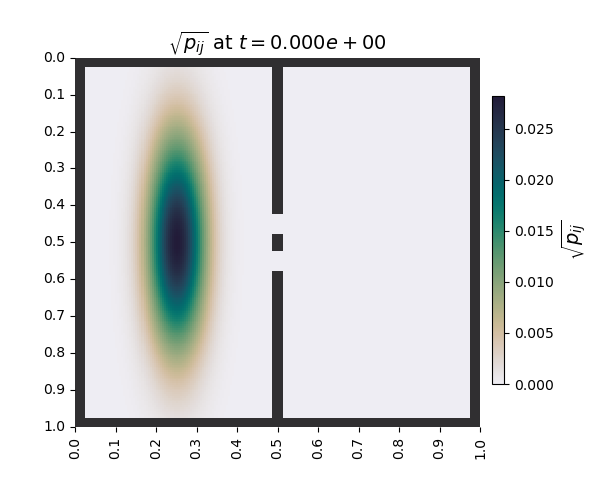
\includegraphics[width=.8\linewidth]{Project 5/figures/problem8and9_M201_Nslits2_sqrtpij_000.png}
    \caption{The square root of the probability at \( t = 0.0 \). Note the color bar scale is different between this figure and Figure \ref{fig:fig2} and \ref{fig:fig3}.}
    \label{fig:fig1}
\end{figure}

\begin{figure}[htbp]
    \centering
    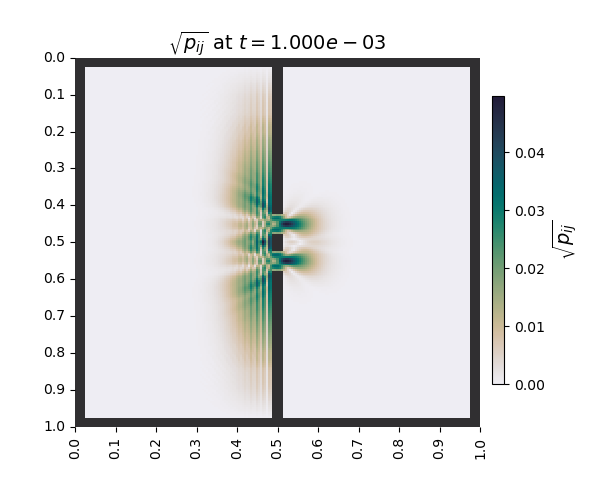
\includegraphics[width=.8\linewidth]{Project 5/figures/problem8and9_M201_Nslits2_sqrtpij_040.png}
    \caption{The square root of the probability at \( t = 0.001 \). Note the color bar scale is different between this figure and Figure \ref{fig:fig1} and \ref{fig:fig3}.}
    \label{fig:fig2}
\end{figure}

\begin{figure}[htbp]
    \centering
    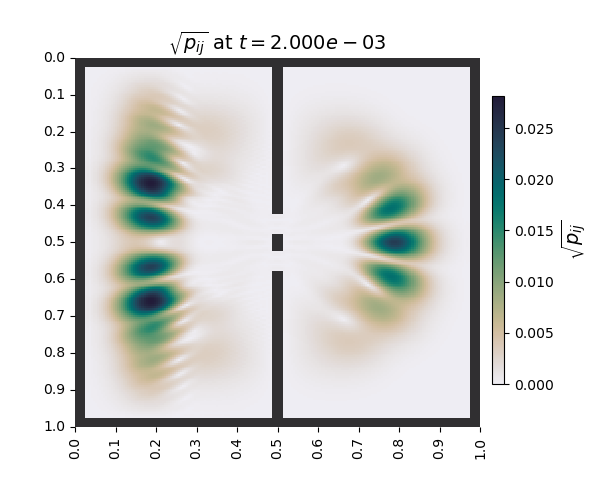
\includegraphics[width=.8\linewidth]{Project 5/figures/problem8and9_M201_Nslits2_sqrtpij_080.png}
    \caption{The square root of the probability at \( t = 0.002 \). Note the color bar scale is different between this figure and Figure \ref{fig:fig1} and \ref{fig:fig2}.}
    \label{fig:fig3}
\end{figure}

Together the figures show how the position probability is reduced as the simulation evolves. Further they show how the incident with the slit transforms the distribution from uni modal to a multi modal distribution. 

Figure \ref{fig:fig3} and \ref{fig:fig3a} show the distribution at $t=0.002$. Creating an imaginary boundary at $x=0.8$ we create the marginal distribution $p(y|x=0.8; t=0.002)$ shown in Figure \ref{fig:marg_2slits}. Combining these three plots we can see; a) that the particle position is uncertain (ref, Heisenberg's uncertainty principle) and  b) the wave nature of the particle as it is incident on a slit wall (ref de Brouglie). 

\begin{figure}[h!]
    \centering
    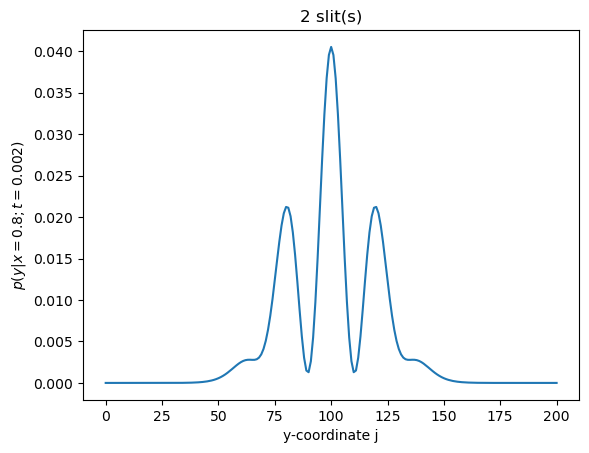
\includegraphics[width=0.8\linewidth]{Project 5/figures/marg_distribution_x08_t0002_Nslits2.png}
    \caption{The marginal distribution $p(y|x=0.8; t=0.002)$ for a double slit setup. Note, this is not the probability $p(x=0.8,y; t=0.002)$ as it is normalized. }
    \label{fig:marg_2slits}
\end{figure}

As a supplement to Figure \ref{fig:marg_2slits} we also include the marginal distributions for the single and triple slit setup in Figures \ref{fig:marg_1slits} and \ref{fig:marg_3slits} respectively. Here we see how the number of slits affect the number of modes expected after being incident on a slit wall. Some key features are that we observe the interference patterns which are expected from observational experiments conducted with multiple particles to construct similar distributions.

\subsection{Future work and improvements}\label{sec:future_work}

For this study the implemented code is not particularly fast. Therefor future work should include a code optimization both in terms of CPU and memory usage. The three first points we should investigate is; 1) the choice of linear algebra solver, which probably slows us down due to the fact that larger amounts of data are actively kept in memory compared to indirect methods, and 2) the effect of I/O operations (opening, saving, etc) and 3) duplicated data in the solver (e.g. storing the diagonal of $A$ and $B$ both in the matrices and as a class parameter. Further, we see that numerical instabilities have a larger prevalence as there are distributional shifts. From a simulation of 320 time steps these do not really accumulate, but a longer control run should also be conducted to see if the simulate is able to adjust back as seems promising from the left panel in Figure \ref{fig:p5_computational_stability}.

\end{document}
